\documentclass[12pt]{article}
\usepackage{setspace}
\usepackage{geometry}
\usepackage{hyperref}
\usepackage{multicol}
\usepackage{booktabs}
\usepackage{amssymb}
\usepackage{graphicx}
\usepackage{caption}
\usepackage{float}


\geometry{margin=1in}
\bibliographystyle{plain}

\title{Hetergoneity in Lifetime Earnings Risk}

\author{Ethan Ballou\thanks{University of Wisconsin - Milwaukee}}


\date{\today}

\begin{document}
\maketitle
\thispagestyle{empty}


%\date{\today}
%\pubMonth{Month}
%\pubYear{Year}
%\pubVolume{Vol}
%\pubIssue{Issue}
%\JEL{}
%\Keywords{}

\begin{abstract}
\begin{singlespace}
\noindent 
Abstract.  This is our abstract.  It is abstract.  
\end{singlespace}
\end{abstract}
\noindent
\textbf{Keywords}: \\
\textbf{JEL Codes}: \\






\clearpage
\setcounter{page}{1}
\begin{center}
%PRELIMINARY: DO NOT CIRCULATE OR QUOTE
\end{center}




\section{Introduction}

This is an example citation \cite{exampleCitation}. \\ 


\section{Literature Review}

\section{Data and Model}

\section{Empirical Strategy}

\section{Results}

\section{Conclusion}




% EDU1 - less than high school
% EDU2 - high school or some college
% EDU3 - bachelor's but less than master's






\begin{figure}[H]
    \centering
    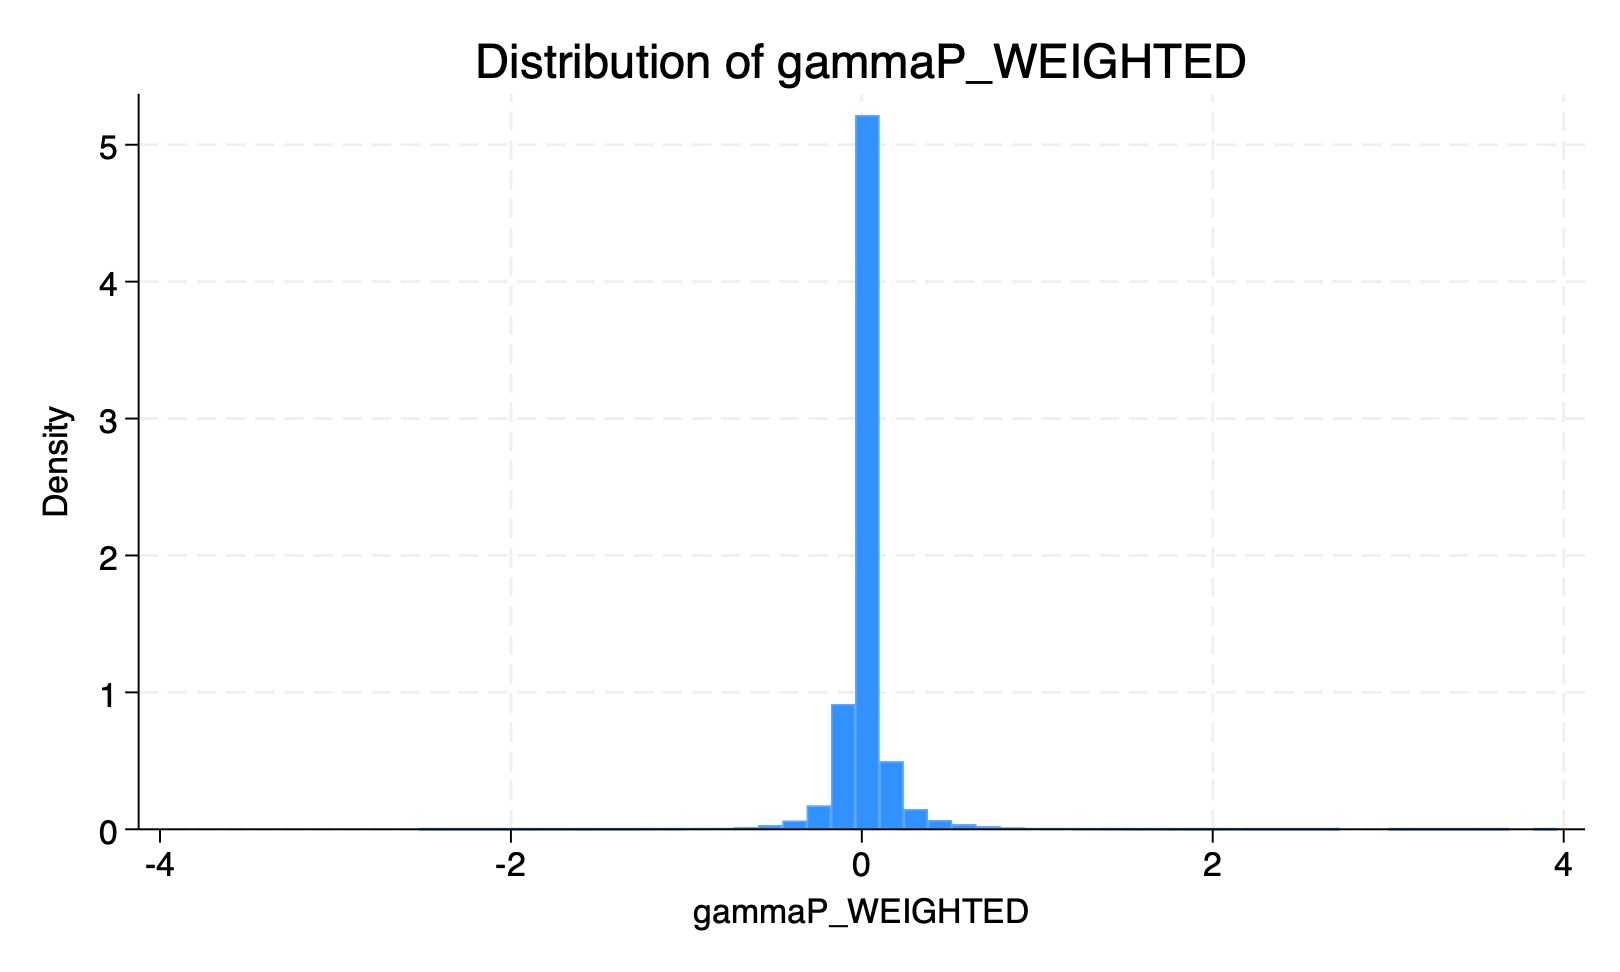
\includegraphics[width=1\textwidth]{/Users/ethanballou/Documents/GitHub/LifetimeEarningsRisk/Plots/histogram_gammaP_WEIGHTED.png}
    \caption{Distribution of gammaP\_WEIGHTED}
\end{figure}



\begin{figure}[H]
    \centering
    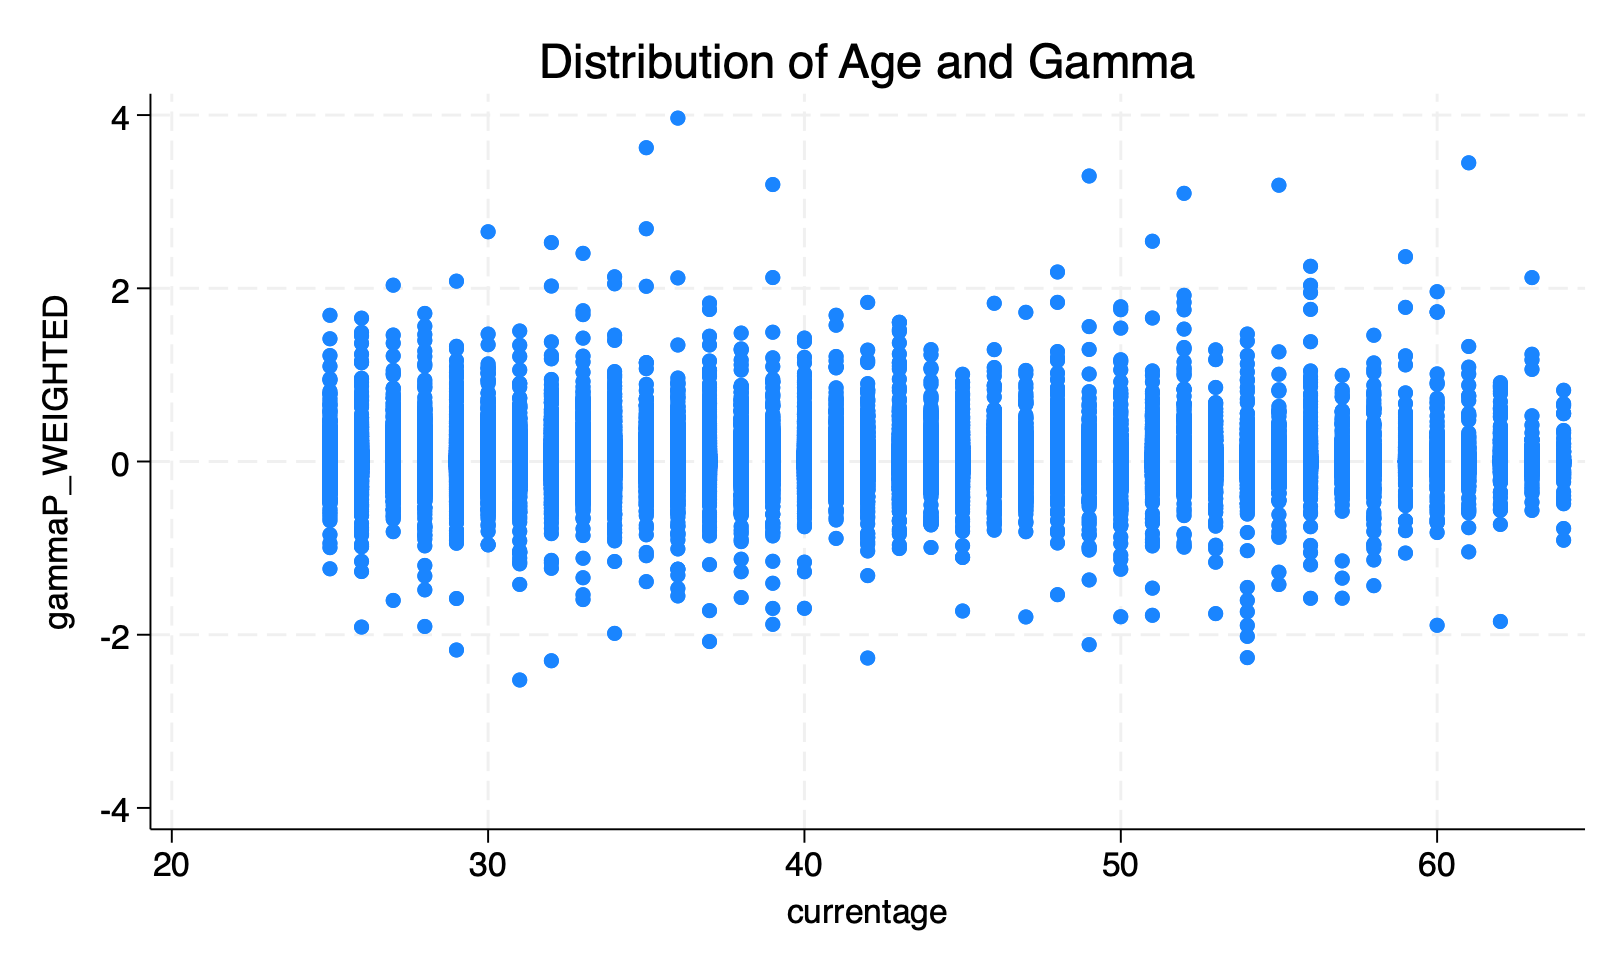
\includegraphics[width=1\textwidth]{/Users/ethanballou/Documents/GitHub/LifetimeEarningsRisk/Plots/scatter_age_gammaP_WEIGHTED.png}
    \caption{Scatterplot of Age vs. gammaP\_WEIGHTED}
\end{figure}




% does the sign matter? Address this 



Gamma is a centered heavily around 0 with a standard deviation of 0.1686 as seen in Figure 1. Being centered at 0 is due to its derivation and as seen in Figure 2 there is not a clear correlation with age which might be expected.


The beginning of the analysis is just simple OLS regressions of gamma. The further analysis will focus on the which variables are most significant or important and less on the actual size of the effect. However size of coefficents is something OLS can easily address. While gamma is centered around zero, variables do still have effects despite being small. Table 1 shows the OLS estimates for gamma across different specifications. 

The different specifications include different sets of controls, such as occupation and industry controls along wiht other controls such as state, year, cohort, and race.

The coefficents are quite small however some are larger than others. Less than high school and high school or some college education are lightly significant in some cases. They have some of the larger effects compared to many of the variables with less than high school being somewhare around -0.004 and -0.006 and highschool and some college being around -0.003 to -0.005. 

The bachelors degree and less than a masters variable is smaller than the other two education variables which would imply college education does provide stabler employment and earnings overall. Howvever despite this the variable is not significant in any of the models suggests larger variation in earnings for those with a bachelor's degree or less than a master's degree. This variation could be due to variation in fields of study which would explain the larger coefficents in models 3, 4, and 5 where industry or occupation controls are included.

% EDU3 and industry interaction? FE regression with industry controls and industry controls with EDU3 interaction

The other variables that are significant are the age variables. The age, age squared, and age cubed varaibles are all significant in all models. The interesting results is that the age squared and cubed variables are slightly more significant than the regular age variable. On some level it is expected that towards the end of a person's career they would become more risk averse and it is possible the squared and cubed terms capture this variation. 

Overall the OLS results show that education and age are important in explaining lifetime earnings risk. This pattern contrinues in the stepwise and lasso results.



TABLE 2 HERE


Table 2 shows the stepwise results for the same 5 models. The stepwise results are based on a p-value threshold of 0.05. The stepsie regression results are able to assign cardinal rankings to how significant certain variables are in explaining lifetime earnings risk. In the stepwise regression the controls are treated as groups of variables such that the model cannot remove single variables from a set of controls and must remove the entire set of controls at once. The numbers assigned to the variables not selected indicate the the order in which they were removed usch that 1 is the last variable removed before the model is finalized.

The stewise models show similar results to OLS in that both education and age play an important role in predicting lifetime earnigns risk. Simlar to OLS less than highschool and high school and some college are the two important to the model while the bachelors degreee and less than a masters is not selected and not relevant in the model. And for the two models where the two important education variables aren't selected they are still the last two variables to be removed before the cutoff. 


The other interesting variables that show up are the probability of recession and real GDP growth. These two variables are in the last 4 variables to be removed in all models suggesting their importance. Specifically probability of recession was the last variable removed in 3 of the models despite different controls. Probability of recession and real GDP growth were both important with and without industry controls which would be where one would expect at least some of their variation to be captured. This implies that variation across industry sensitivity to macroeconomic outcomes may not actually have much explanatory power in lifetime earnings risk.

Some surprising results regarding items not in the model is that industry controls are not selected by the stepwise regression in either of the models it is included in. This is despite the first model not including occupation controls.


Table 2 shows the stepwise estimates of gamma using the different specifications. 

- Similar to OLS, All the age variables have explnatory power, and EDU1 and EDU2 are mildy explanatory in some cases.
- Occupation and state controls are selected in all cases
- Probability of recession, and real GDP growth, are top 4 every time
- veteran, wages, and many of the controls are seen as the least important variables in just about all the models  



% report mse or r2

Table 3 shows the lasso of gamma using the different specifications. 

- The are quite different from the stepwise results. All controls are selected in all cases
- PrRecess and rGDPgrow are not selected in any case across lambda values except in the first model
- Non of the continuous variables are selected in any of the models once the optimal lambda is selected by cv 
- Howvever the EDU1 and EDU2 are the most important varaibles after the selected varaibles in most cases
- MA5 and OLF are also quite strong and come after EDU1 and EDU2 in most cases
- In the lasso models the age varaibles aren't selected and in some cases are the last variables considered across lambda values

















\vspace{4cm}







\begin{table}[H]
\centering
\caption{OLS Estimates for $\gamma$ (Coefficients $\times$ 100)}

\begin{tabular}{lccccc}

\toprule
                    & (1)     & (2)   & (3)    & (4)      & (5)         \\
\midrule
Education (less than 12)                & $-0.361$  & $-0.360$    & $-0.522^{*}$  & $-0.597^{*}$   & $-0.630^{**}$    \\
                    & (0.255)   & (0.273)     & (0.286)   & (0.307)    & (0.310)     \\
Education (12 to 14)                & $-0.283$  & $-0.315^{*}$    & $-0.418^{**}$  & $-0.417^{*}$   & $-0.455^{**}$    \\
                    & (0.175)   & (0.181)     & (0.193)   & (0.216)    & (0.219)     \\
Education (14 to 16)                & $-0.089$  & $-0.063$    & $-0.138$  & $-0.114$   & $-0.147$    \\
                    & (0.206)   & (0.209)     & (0.216)   & (0.228)    & (0.230)     \\
PrRecess            & $-0.006$   & $-0.038$     & $-0.037$   & $-0.040$    & $-0.039$     \\
                    & (0.005)   & (0.036)     & (0.036)   & (0.036)    & (0.036)     \\
rGDPgrow            & $-0.033$   & $0.076$     & $0.071$   & $0.063$    & $0.058$     \\
                    & (0.033)   & (0.172)     & (0.172)   & (0.172)    & (0.172)     \\
fhwage0\_P0         & $-0.006$   & $0.004$     & $0.005$   & $0.002$    & $0.004$     \\
                    & (0.025)   & (0.027)     & (0.027)   & (0.028)    & (0.028)     \\
ma5aep              & $0.004$   & $0.003$     & $0.004$   & $0.004$    & $0.004$     \\
                    & (0.003)   & (0.003)     & (0.003)   & (0.003)    & (0.004)     \\
veteran             & $0.021$   & $-0.003$     & $0.053$   & $0.018$    & $0.040$     \\
                    & (0.141)   & (0.151)     & (0.153)   & (0.154)    & (0.155)     \\
OLF                 & $0.627$   & $0.584$     & $0.550$   & $0.619$    & $0.625$     \\
                    & (0.627)   & (0.628)     & (0.628)   & (0.629)    & (0.629)     \\
tenure              & $-0.010$   & $-0.009$     & $-0.008$   & $-0.012$    & $-0.010$     \\
                    & (0.011)   & (0.012)     & (0.012)   & (0.012)    & (0.012)     \\
currentage          & $0.874^{**}$   & $0.936^{**}$     & $0.926^{**}$   & $0.919^{**}$    & $0.907^{**}$     \\
                    & (0.380)   & (0.384)     & (0.385)   & (0.385)    & (0.385)     \\
currentagesq        & $-0.023^{**}$  & $-0.025^{***}$    & $-0.025^{***}$  & $-0.025^{***}$   & $-0.024^{***}$    \\
                    & (0.009)   & (0.009)     & (0.009)   & (0.009)    & (0.009)     \\
currentagecube      & $0.0002^{***}$  & $0.0002^{***}$    & $0.0002^{***}$  & $0.0002^{***}$   & $0.0002^{***}$    \\
                    & (0.0001)   & (0.0001)     & (0.0001)   & (0.0001)    & (0.0001)     \\

\midrule
Occupation Controls  &               &                 &               & \checkmark    & \checkmark     \\
Industry Controls    &               &                 & \checkmark    &               & \checkmark     \\
Other Controls      &               & \checkmark      & \checkmark    & \checkmark    & \checkmark     \\
\bottomrule
\end{tabular}%
\newline
\textit{Notes:} Standard errors in parentheses. Other controls include state, year, race, and cohort fixed effects. Statistical significance: $^{*}p<0.10$, $^{**}p<0.05$, $^{***}p<0.01$. All coefficients and standard errors are multiplied by 100 for easier interpretation.

\end{table}






\begin{table}[H]
\centering
\caption{Stepwise Results for $\gamma$}

\begin{tabular}{lccccc}

\toprule
                    & (1)     & (2)   & (3)    & (4)      & (5)         \\

\midrule
EDU1                & selected  & 2    & 2  & selected   & selected    \\
EDU2                & selected  & 1    & 1  & selected   & selected    \\
EDU3                & 6  & 10    & 8  & 6   & 6    \\
PrRecess            & 1   & 3     & 3   & 1    & 1     \\
rGDPgrow            & 4   & 4     & 4   & 4    & 4     \\
fhwage0\_P0         & 7   & 11     & 13   & 9    & 9     \\
ma5aep              & 2   & 6     & 6   & 3    & 3     \\
veteran             & 8   & 12     & 12   & 10    & 11     \\
OLF                 & 3   & 5     & 5   & 2    & 2     \\
tenure              & 5   & 7     & 9   & 5    & 5     \\
currentage          & selected   & selected     & selected   & selected    & selected     \\
currentagesq        & selected  & selected    & selected  & selected   & selected    \\
currentagecube      & selected  & selected    & selected  & selected   & selected    \\

\midrule
Occupation Controls      & -   & -    & -  & selected   & selected    \\
Industry Controls      & -  & -    & 7  & -   & 10    \\
Cohort Controls      & -  & 8    & 10  & 7   & 7    \\
Race Controls      & -  & 13    & 14  & 11   & 12    \\
Year Controls      & -  & 9    & 11  & 8   & 8    \\
State Controls      & -  & selected    & selected  & selected   & selected    \\

\midrule
Occupation Controls  &               &                 &               & \checkmark    & \checkmark     \\
Industry Controls    &               &                 & \checkmark    &               & \checkmark     \\
Other Controls      &               & \checkmark      & \checkmark    & \checkmark    & \checkmark     \\

\bottomrule
\end{tabular}%
\newline

\footnotesize
\textit{Notes:} This table reports results from stepwise regression models using a p-value threshold of 0.05. "Selected" indicates variables retained in the final model. Numbers indicate the order of variable removal (with 1 being the last variable removed before model finalization). "-" indicates the variable was not included in the initial model specification.

\end{table}





\begin{table}[H]
\centering
\caption{Lasso Results for $\gamma$}

\begin{tabular}{lccccc}

\toprule
                    & (1)     & (2)   & (3)    & (4)      & (5)         \\

\midrule
EDU1                &  3  &  3    &  2  &  1   &  1    \\
EDU2                &  2  &  1    &  1  &  1   &  1    \\
EDU3                &  8  &  7    &  6  &  6   &  4    \\
PrRecess            &  4    & Not Selected    & Not Selected   & Not Selected    & Not Selected     \\
rGDPgrow            &  6    & Not Selected     & Not Selected   & Not Selected    & Not Selected     \\
fhwage0\_P0         &  7   &  9     &  9   &  8    &  6     \\
ma5aep              &  1   &  2     &  1   &  2    &  1     \\
veteran             &  10   &  8     &  8   &  7    &  5     \\
OLF                 &  3   &  2     &  3   &  1    &  1     \\
tenure              &  5   &  4     &  4   &  3    &  2     \\
currentage          &  9   &  6     &  7   &  5    &  4     \\
currentagesq        &  11  &  10    &  10  &  8   &  7    \\
currentagecube      &  2  &  5    &  5  &  4   &  3    \\

\midrule
Occupation Controls      & -   & -    & -  & Selected   & Selected    \\
Industry Controls      & -  & -    & Selected  & -   & Selected    \\
Cohort Controls      & -  & Selected    & Selected  & Selected   & Selected    \\
Race Controls      & -  & Selected    & Selected  & Selected   & Selected    \\
Year Controls      & -  & Selected    & Selected  & Selected   & Selected    \\
State Controls      & -  & Selected    & Selected  & Selected   & Selected    \\


\midrule
Occupation Controls  &               &                 &               & \checkmark    & \checkmark     \\
Industry Controls    &               &                 & \checkmark    &               & \checkmark     \\
Other Controls      &               & \checkmark      & \checkmark    & \checkmark    & \checkmark     \\

\bottomrule
\end{tabular}%
\newline

\footnotesize
\textit{Notes:} This table reports variables selected by Lasso regression with Bayesian Information Criterion (BIC) variable selection. "Selected" indicates variables retained in the final model. Numbers in parentheses indicate the order in which variables were added to the model. "-" indicates the variable was not included. "Not Selected" indicates the variable was not selected by Lasso but was provided in the model specification.

\end{table}








\begin{table}[H]
\centering
\caption{Lasso and SHAP Results for Occupations}

\footnotesize  % Controls the font size of the table content

\begin{tabular}{lcc|lcc}
\toprule
Occupation & SHAP Rank & LASSO Rank & Occupation & SHAP Rank & LASSO Rank \\
\midrule
occ\_21 & 1 & Not Selected & occ\_60 & 2 & 16 \\
occ\_84 & 3 & 26 & occ\_61 & 4 & 13 \\
occ\_1 & 5 & 14 & occ\_45 & 6 & 20 \\
occ\_70 & 7 & Not Selected & occ\_98 & 8 & 14 \\
occ\_37 & 9 & Not Selected & occ\_97 & 10 & 27 \\
occ\_2 & 11 & 20 & occ\_99 & 12 & 22 \\
occ\_13 & 13 & 14 & occ\_9 & 14 & 24 \\
occ\_11 & 15 & 23 & occ\_83 & 16 & 21 \\
occ\_4 & 17 & 3 & occ\_101 & 18 & Not Selected \\
occ\_95 & 19 & 25 & occ\_79 & 20 & 15 \\
occ\_85 & 21 & Not Selected & occ\_6 & 22 & 8 \\
occ\_999 & 23 & Not Selected & occ\_8 & 24 & Not Selected \\
occ\_93 & 25 & 17 & occ\_55 & 26 & 21 \\
occ\_20 & 27 & 16 & occ\_53 & 28 & 23 \\
occ\_17 & 29 & 6 & occ\_19 & 30 & Not Selected \\
occ\_5 & 31 & 18 & occ\_40 & 32 & 23 \\
occ\_58 & 33 & 26 & occ\_34 & 34 & 19 \\
occ\_59 & 35 & 13 & occ\_7 & 36 & Not Selected \\
occ\_77 & 37 & 21 & occ\_87 & 38 & 21 \\
occ\_50 & 39 & 19 & occ\_14 & 40 & Not Selected \\
occ\_54 & 41 & 28 & occ\_96 & 42 & 15 \\
occ\_38 & 43 & 20 & occ\_3 & 44 & 12 \\
occ\_15 & 45 & 14 & occ\_32 & 46 & 14 \\
occ\_18 & 47 & 11 & occ\_42 & 48 & 11 \\
occ\_73 & 49 & Not Selected & occ\_31 & 50 & Not Selected \\
occ\_62 & 51 & 21 & occ\_44 & 52 & 17 \\
occ\_33 & 53 & 19 & occ\_63 & 54 & 28 \\
occ\_49 & 55 & 18 & occ\_86 & 56 & 17 \\
occ\_36 & 57 & Not Selected & occ\_43 & 58 & 16 \\
occ\_39 & 59 & Not Selected & occ\_74 & 60 & 17 \\
occ\_72 & 61 & Not Selected & occ\_64 & 62 & 2 \\
occ\_56 & 63 & Not Selected & occ\_92 & 64 & Not Selected \\
occ\_80 & 65 & Not Selected & occ\_88 & 66 & 13 \\
occ\_12 & 67 & 14 & occ\_75 & 68 & 25 \\
occ\_81 & 69 & Not Selected & occ\_30 & 70 & Not Selected \\
occ\_35 & 71 & 9 & occ\_57 & 72 & Not Selected \\
occ\_89 & 73 & Not Selected & occ\_71 & 74 & Not Selected \\
occ\_16 & 75 & 29 & occ\_94 & 76 & 25 \\
occ\_82 & 77 & Not Selected & occ\_52 & 78 & Not Selected \\
\bottomrule
\end{tabular}%
\newline

\footnotesize
\textit{Notes:} This table reports occupations selected by Lasso regression with Bayesian Information Criterion (BIC) for predicting earnings risk. "SHAP Rank" shows the variable importance ranking based on SHAP values (lower numbers indicate greater importance). "LASSO Order" indicates the order in which variables would enter the model if the penalty were relaxed. Note that the BIC-optimal model contained no occupation variables.

\end{table}











\begin{table}[H]
\centering

\caption{Lasso and SHAP Results for Industries}

\begin{tabular}{lcc}

\toprule
Industry & SHAP Rank & LASSO Rank\\
\midrule
twoind\_3 & 1 & 28 \\
twoind\_9 & 2 & 10 \\
twoind\_19 & 3 & 18 \\
twoind\_30 & 4 & 2 \\
twoind\_16 & 5 & 19 \\
twoind\_21 & 6 & 8 \\
twoind\_14 & 7 & Not Selected \\
twoind\_18 & 8 & Not Selected \\
twoind\_5 & 9 & 7 \\
twoind\_33 & 10 & 3 \\
twoind\_10 & 11 & 21 \\
twoind\_4 & 12 & 27 \\
twoind\_29 & 13 & 21 \\
twoind\_999 & 14 & 17 \\
twoind\_15 & 15 & 16 \\
twoind\_7 & 16 & 13 \\
twoind\_11 & 17 & 16 \\
twoind\_12 & 18 & 3 \\
twoind\_22 & 19 & 27 \\
twoind\_1 & 20 & 11 \\
twoind\_25 & 21 & 10 \\
twoind\_27 & 22 & 3 \\
twoind\_6 & 23 & 23 \\
twoind\_20 & 24 & 11 \\
twoind\_23 & 25 & 18 \\
twoind\_8 & 26 & 28 \\
twoind\_24 & 27 & 29 \\
twoind\_31 & 28 & 23 \\
twoind\_28 & 29 & 7 \\
twoind\_13 & 30 & 25 \\
\bottomrule
\end{tabular}%
\newline

\footnotesize
\textit{Notes:} This table reports industries selected by Lasso regression with Bayesian Information Criterion (BIC) for predicting earnings risk. "LASSO Selection Order" indicates the order in which variables would enter the model if the penalty were relaxed. "SHAP Ranking" shows the variable importance ranking based on SHAP values (lower numbers indicate greater importance). Note that the BIC-optimal model contained no industry variables.

\end{table}







\begin{figure}[H]
    \centering
    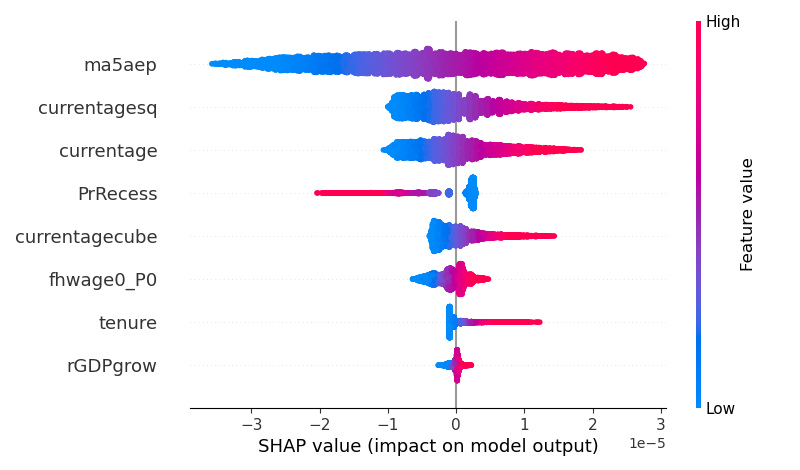
\includegraphics[width=1\textwidth]{/Users/ethanballou/Documents/GitHub/LifetimeEarningsRisk/Plots/ShapSummaryPlot.png}
    \caption{SHAP Summary Plot}
\end{figure}



\begin{figure}[H]
    \centering
    \begin{minipage}{0.49\textwidth}
        \centering
        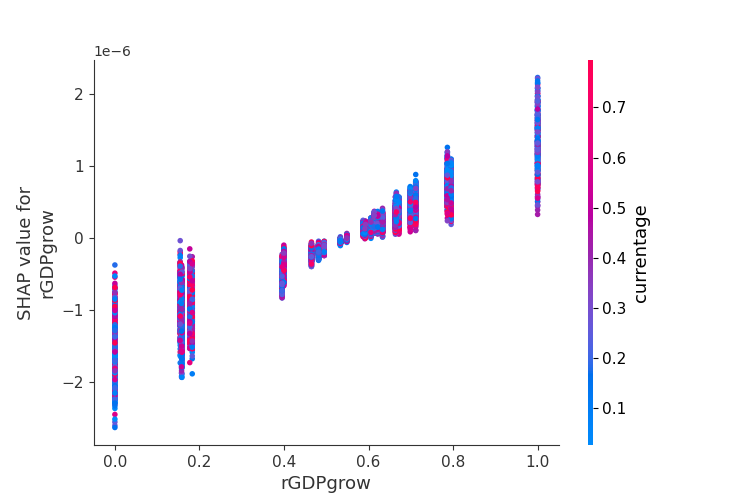
\includegraphics[width=\textwidth]{/Users/ethanballou/Documents/GitHub/LifetimeEarningsRisk/Plots/GDP_Age.png}
        \caption{GDP by Age}
    \end{minipage}
    \hfill
    \begin{minipage}{0.49\textwidth}
        \centering
        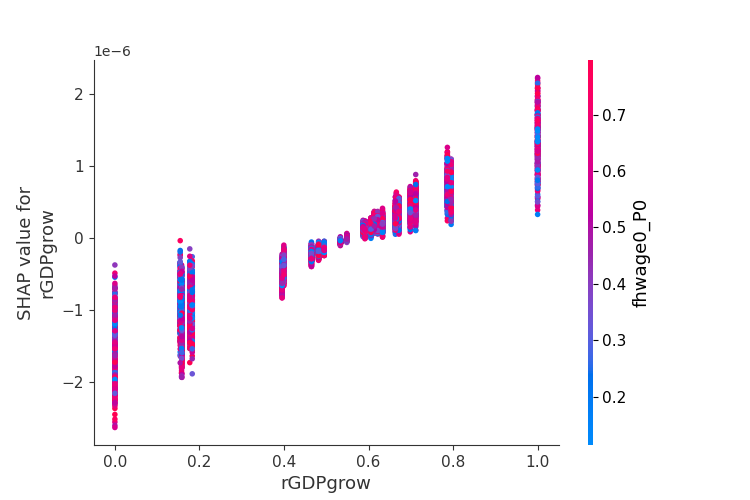
\includegraphics[width=\textwidth]{/Users/ethanballou/Documents/GitHub/LifetimeEarningsRisk/Plots/GDP_Income.png}
        \caption{GDP by Income}
    \end{minipage}
\end{figure}






\bibliography{references}

\end{document}